% Options for packages loaded elsewhere
% Options for packages loaded elsewhere
\PassOptionsToPackage{unicode}{hyperref}
\PassOptionsToPackage{hyphens}{url}
\PassOptionsToPackage{dvipsnames,svgnames,x11names}{xcolor}
%
\documentclass[
]{agujournal2019}
\usepackage{xcolor}
\usepackage{amsmath,amssymb}
\setcounter{secnumdepth}{5}
\usepackage{iftex}
\ifPDFTeX
  \usepackage[T1]{fontenc}
  \usepackage[utf8]{inputenc}
  \usepackage{textcomp} % provide euro and other symbols
\else % if luatex or xetex
  \usepackage{unicode-math} % this also loads fontspec
  \defaultfontfeatures{Scale=MatchLowercase}
  \defaultfontfeatures[\rmfamily]{Ligatures=TeX,Scale=1}
\fi
\usepackage{lmodern}
\ifPDFTeX\else
  % xetex/luatex font selection
\fi
% Use upquote if available, for straight quotes in verbatim environments
\IfFileExists{upquote.sty}{\usepackage{upquote}}{}
\IfFileExists{microtype.sty}{% use microtype if available
  \usepackage[]{microtype}
  \UseMicrotypeSet[protrusion]{basicmath} % disable protrusion for tt fonts
}{}
\makeatletter
\@ifundefined{KOMAClassName}{% if non-KOMA class
  \IfFileExists{parskip.sty}{%
    \usepackage{parskip}
  }{% else
    \setlength{\parindent}{0pt}
    \setlength{\parskip}{6pt plus 2pt minus 1pt}}
}{% if KOMA class
  \KOMAoptions{parskip=half}}
\makeatother
% Make \paragraph and \subparagraph free-standing
\makeatletter
\ifx\paragraph\undefined\else
  \let\oldparagraph\paragraph
  \renewcommand{\paragraph}{
    \@ifstar
      \xxxParagraphStar
      \xxxParagraphNoStar
  }
  \newcommand{\xxxParagraphStar}[1]{\oldparagraph*{#1}\mbox{}}
  \newcommand{\xxxParagraphNoStar}[1]{\oldparagraph{#1}\mbox{}}
\fi
\ifx\subparagraph\undefined\else
  \let\oldsubparagraph\subparagraph
  \renewcommand{\subparagraph}{
    \@ifstar
      \xxxSubParagraphStar
      \xxxSubParagraphNoStar
  }
  \newcommand{\xxxSubParagraphStar}[1]{\oldsubparagraph*{#1}\mbox{}}
  \newcommand{\xxxSubParagraphNoStar}[1]{\oldsubparagraph{#1}\mbox{}}
\fi
\makeatother


\usepackage{longtable,booktabs,array}
\usepackage{calc} % for calculating minipage widths
% Correct order of tables after \paragraph or \subparagraph
\usepackage{etoolbox}
\makeatletter
\patchcmd\longtable{\par}{\if@noskipsec\mbox{}\fi\par}{}{}
\makeatother
% Allow footnotes in longtable head/foot
\IfFileExists{footnotehyper.sty}{\usepackage{footnotehyper}}{\usepackage{footnote}}
\makesavenoteenv{longtable}
\usepackage{graphicx}
\makeatletter
\newsavebox\pandoc@box
\newcommand*\pandocbounded[1]{% scales image to fit in text height/width
  \sbox\pandoc@box{#1}%
  \Gscale@div\@tempa{\textheight}{\dimexpr\ht\pandoc@box+\dp\pandoc@box\relax}%
  \Gscale@div\@tempb{\linewidth}{\wd\pandoc@box}%
  \ifdim\@tempb\p@<\@tempa\p@\let\@tempa\@tempb\fi% select the smaller of both
  \ifdim\@tempa\p@<\p@\scalebox{\@tempa}{\usebox\pandoc@box}%
  \else\usebox{\pandoc@box}%
  \fi%
}
% Set default figure placement to htbp
\def\fps@figure{htbp}
\makeatother


% definitions for citeproc citations
\NewDocumentCommand\citeproctext{}{}
\NewDocumentCommand\citeproc{mm}{%
  \begingroup\def\citeproctext{#2}\cite{#1}\endgroup}
\makeatletter
 % allow citations to break across lines
 \let\@cite@ofmt\@firstofone
 % avoid brackets around text for \cite:
 \def\@biblabel#1{}
 \def\@cite#1#2{{#1\if@tempswa , #2\fi}}
\makeatother
\newlength{\cslhangindent}
\setlength{\cslhangindent}{1.5em}
\newlength{\csllabelwidth}
\setlength{\csllabelwidth}{3em}
\newenvironment{CSLReferences}[2] % #1 hanging-indent, #2 entry-spacing
 {\begin{list}{}{%
  \setlength{\itemindent}{0pt}
  \setlength{\leftmargin}{0pt}
  \setlength{\parsep}{0pt}
  % turn on hanging indent if param 1 is 1
  \ifodd #1
   \setlength{\leftmargin}{\cslhangindent}
   \setlength{\itemindent}{-1\cslhangindent}
  \fi
  % set entry spacing
  \setlength{\itemsep}{#2\baselineskip}}}
 {\end{list}}
\usepackage{calc}
\newcommand{\CSLBlock}[1]{\hfill\break\parbox[t]{\linewidth}{\strut\ignorespaces#1\strut}}
\newcommand{\CSLLeftMargin}[1]{\parbox[t]{\csllabelwidth}{\strut#1\strut}}
\newcommand{\CSLRightInline}[1]{\parbox[t]{\linewidth - \csllabelwidth}{\strut#1\strut}}
\newcommand{\CSLIndent}[1]{\hspace{\cslhangindent}#1}



\setlength{\emergencystretch}{3em} % prevent overfull lines

\providecommand{\tightlist}{%
  \setlength{\itemsep}{0pt}\setlength{\parskip}{0pt}}



 


\usepackage{url} %this package should fix any errors with URLs in refs.
\usepackage{lineno}
\usepackage[inline]{trackchanges} %for better track changes. finalnew option will compile document with changes incorporated.
\usepackage{soul}
\linenumbers
\makeatletter
\@ifpackageloaded{caption}{}{\usepackage{caption}}
\AtBeginDocument{%
\ifdefined\contentsname
  \renewcommand*\contentsname{Table of contents}
\else
  \newcommand\contentsname{Table of contents}
\fi
\ifdefined\listfigurename
  \renewcommand*\listfigurename{List of Figures}
\else
  \newcommand\listfigurename{List of Figures}
\fi
\ifdefined\listtablename
  \renewcommand*\listtablename{List of Tables}
\else
  \newcommand\listtablename{List of Tables}
\fi
\ifdefined\figurename
  \renewcommand*\figurename{Figure}
\else
  \newcommand\figurename{Figure}
\fi
\ifdefined\tablename
  \renewcommand*\tablename{Table}
\else
  \newcommand\tablename{Table}
\fi
}
\@ifpackageloaded{float}{}{\usepackage{float}}
\floatstyle{ruled}
\@ifundefined{c@chapter}{\newfloat{codelisting}{h}{lop}}{\newfloat{codelisting}{h}{lop}[chapter]}
\floatname{codelisting}{Listing}
\newcommand*\listoflistings{\listof{codelisting}{List of Listings}}
\makeatother
\makeatletter
\makeatother
\makeatletter
\@ifpackageloaded{caption}{}{\usepackage{caption}}
\@ifpackageloaded{subcaption}{}{\usepackage{subcaption}}
\makeatother
\usepackage{bookmark}
\IfFileExists{xurl.sty}{\usepackage{xurl}}{} % add URL line breaks if available
\urlstyle{same}
\hypersetup{
  pdftitle={DNA methylation in Mytilus chilensis},
  pdfkeywords={DNA methylation, Mytilus
chilensis, epigenetics, adaptation, aquaculture},
  colorlinks=true,
  linkcolor={blue},
  filecolor={Maroon},
  citecolor={Blue},
  urlcolor={Blue},
  pdfcreator={LaTeX via pandoc}}



\draftfalse

\begin{document}
\title{DNA methylation in Mytilus chilensis}

\authors{Cristian Gallardo\affil{1}, Valentina
Venezuala\affil{1}, Steven Roberts\affil{2}}
\affiliation{1}{University of Concepcion, }\affiliation{2}{University of
Washington, }
\correspondingauthor{Cristian
Gallardo}{cgallardo@udec.cl}\correspondingauthor{Valentina
Venezuala}{vvenezuala@udec.cl}\correspondingauthor{Steven
Roberts}{sr320@uw.edu}


\begin{abstract}
We investigate genome-wide DNA methylation patterns in Mytilus chilensis
from two contrasting seedbeds---Cochamó and Yaldad---using whole-genome
bisulfite sequencing and high-throughput bioinformatics. We identify
1117 differentially methylated loci (DMLs) and genes, revealing a shift
toward hypomethylation among DML-associated genes. Functional annotation
shows that DMLs are concentrated in genes mediating metabolism,
development, and cellular organization, with many targets localized to
cytoplasmic and nuclear compartments. DML-associated genes are dispersed
across diverse KEGG pathways and contain a wide array of regulatory and
interaction-rich Pfam domains. These findings suggest a system-wide
epigenetic response, with potential consequences for metabolic control
and developmental programming, and provide new insights into how
environmental and anthropogenic forces shape genomic and epigenomic
variation in a key aquaculture species.
\end{abstract}

\section*{Plain Language Summary}
This study explores how DNA methylation may help Chilean blue mussels
adapt to different environments, providing insights for aquaculture and
conservation.




\section{Introduction}\label{introduction}

Understanding how marine species respond to environmental heterogeneity
is critical for conserving locally adapted populations and sustaining
aquaculture practices in the face of global change. The Chilean blue
mussel, Mytilus chilensis, a key endemic species in southern Chile,
supports one of the world's largest mussel aquaculture industries.
However, the biological foundation of population-level adaptation in
this species remains underexplored. Emerging evidence suggests that both
genetic and epigenetic mechanisms---particularly DNA methylation---may
contribute to phenotypic plasticity and local adaptation in marine
invertebrates.

Previous studies have revealed extensive transcriptomic and
mitochondrial differences between M. chilensis populations from
ecologically distinct seedbeds, such as Cochamó (41°S) and Yaldad
(43°S), in the inner sea of Chiloé Island. These differences include
differential expression of genes involved in immunity, metabolism, and
cellular stress responses, as well as tissue-specific shifts in
mitochondrial gene expression linked to local environmental pressures,
including aquaculture practices and variable oxygenation levels (Yévenes
et al., 2021, 2022). Experimental evidence from reciprocal transplants
shows population-specific transcriptional responses and reduced growth
performance upon translocation, highlighting functional divergence
between seedbeds despite high larval connectivity (Yévenes et al.,
2025).

In addition to gene expression differences, recent work has uncovered
epigenetic signatures that may contribute to adaptive divergence. Long
non-coding RNAs (lncRNAs) were found to be differentially expressed
between Cochamó and Yaldad populations, with associated changes in
immune and metabolic gene networks (Yévenes et al., 2023). These
findings underscore the potential for environmentally responsive
regulatory elements---including DNA methylation---to mediate local
adaptation.

Yet, the role of DNA methylation in shaping population-specific
responses in M. chilensis remains unexplored. DNA methylation, a
heritable and reversible epigenetic modification, can influence gene
expression and phenotypic traits without altering the underlying DNA
sequence. In bivalves, DNA methylation is known to affect developmental
and immune processes and may be responsive to environmental stressors
such as hypoxia, toxins, and acidification---conditions that vary across
the Chilean inner sea and have been shown to modulate gene expression
and microbiota composition in M. chilensis (Castillo et al., 2017;
Montúfar-Romero et al., 2024, 2025).

In this study, we investigate genome-wide DNA methylation patterns in
Mytilus chilensis from two contrasting seedbeds---Cochamó and
Yaldad---with the aim of identifying differentially methylated regions
(DMRs) that may underlie local adaptation. By integrating this
epigenetic information with known patterns of gene expression and
environmental context, we seek to illuminate the molecular basis of
ecological divergence and contribute new insights into how environmental
and anthropogenic forces shape genomic and epigenomic variation in a key
aquaculture species.

\section{Methods}\label{methods}

To investigate DNA methylation differences between populations of
Mytilus chilensis from Cochamó and Yaldad, whole-genome bisulfite
sequencing (WGBS) was performed and analyzed using a reproducible,
high-throughput bioinformatics workflow. DNA was extracted from gill
tissue of adult individuals and subjected to bisulfite treatment and
library preparation. Libraries were sequenced on an Illumina NovaSeq
6000 platform, generating 150 bp paired-end reads, with each sample
yielding approximately 120--160 million read pairs, providing
\textgreater30× average coverage across the 1.93 Gb M. chilensis genome.

\subsection{Read Processing and
Alignment}\label{read-processing-and-alignment}

Raw sequencing reads were processed using the nf-core/methylseq pipeline
(version 2.5), implemented through Nextflow (version 23.04.1). Reads
were aligned to the M. chilensis reference genome
(MchilensisGenomeV1.fa), a chromosome-level assembly comprising 14
scaffolds (Gallardo-Escárate et al.~2023), using Bismark (version
0.24.1) with the Bowtie2 aligner (version 2.5.1). Quality trimming was
applied to reverse reads by hard-clipping the final 10 bases (--clip\_r2
10) to mitigate low-quality base calls at the 3′ end. Methylation calls
were extracted using the Bismark methylation extractor and aggregated by
cytosine context. Pipeline execution was configured via a custom .config
file to specify HPC resources and run with --resume, --with-trace,
--with-report, and --with-timeline flags for reproducibility and
tracking. Output files were stored in a structured directory and
included per-base CpG methylation calls, quality control metrics, and
coverage files.

\subsection{Methylation Data Processing and
Filtering}\label{methylation-data-processing-and-filtering}

Downstream analysis was performed in R (version 4.3.1) using the
methylKit package (version 1.10.0). Due to compatibility issues with
newer versions of supporting libraries, data.table was pinned to version
1.14.10. Methylation coverage files were imported using methRead() with
the pipeline = ``bismarkCoverage'' parameter and CpG context specified.
Six samples---three each from Cochamó (LCo\_BSr1--3) and Yaldad
(LYa\_BSr1--3)---were analyzed. Samples were assigned to treatment
groups with Cochamó designated as the control (treatment = 0) and Yaldad
as the treatment group (treatment = 1).

To ensure data quality, CpG sites were filtered to retain only those
with a minimum read coverage of 10 in all samples, excluding those in
the top 2\% of coverage values to reduce PCR bias. Sites were then
unified across samples using unite() with min.per.group = 3 and destrand
= FALSE to retain strand-specific methylation information.

\subsubsection{Exploratory and Differential Methylation
Analyses}\label{exploratory-and-differential-methylation-analyses}

Global methylation patterns were assessed using hierarchical clustering
(Ward's method on correlation distance) and principal component analysis
(PCA) to evaluate sample similarity. Population-level differences in DNA
methylation were then tested using methylKit's logistic regression
model, incorporating a multinomial overdispersion correction
(overdispersion = ``MN'') to account for biological variability.
Statistical testing was performed using the Chi-squared test (test =
``Chisq''), and q-values were adjusted for multiple testing using the
SLIM method (adjust = ``SLIM'').

Differentially methylated loci (DMLs) were defined as CpG sites with an
absolute methylation difference ≥25\% and FDR-adjusted q-value ≤ 0.05.
Separate sets of DMLs were extracted to identify hypomethylated (lower
in Yaldad) and hypermethylated (higher in Yaldad) loci. Results were
saved as tab-delimited text files for downstream annotation and
visualization.

\section{Results}\label{results}

Bisulfite sequencing across six libraries yielded approximately 99.8
million reads per sample. Alignment to the reference genome was
successful for 60.5--61.4\% of reads, with 22--24\% unaligned and
15--16\% aligning ambiguously. After removal of duplicate reads
(2.2--3.5 million per sample), 57.0--58.8 million uniquely aligned reads
remained for methylation analysis.

Genome-wide cytosine methylation was assessed in CpG, CHG, and CHH
contexts. Across samples, \textasciitilde2.1--2.2 billion cytosines were
examined. CpG methylation was the most prominent, with an average of
\textasciitilde36 million methylated CpGs and \textasciitilde205 million
unmethylated CpGs per sample, corresponding to a methylation rate of
approximately 15\%. In contrast, CHG and CHH methylation was much lower,
with methylation levels below 1\% in both contexts. These patterns are
consistent with expectations for invertebrate methylomes, where
methylation is primarily restricted to CpG sites.

In total, 1117 differentially methylated loci (DMLs) were identified
(see Methods and Supplementary Data). These DMLs were distributed across
all chromosomes and classified as either hypomethylated or
hypermethylated based on methylation difference.

\pandocbounded{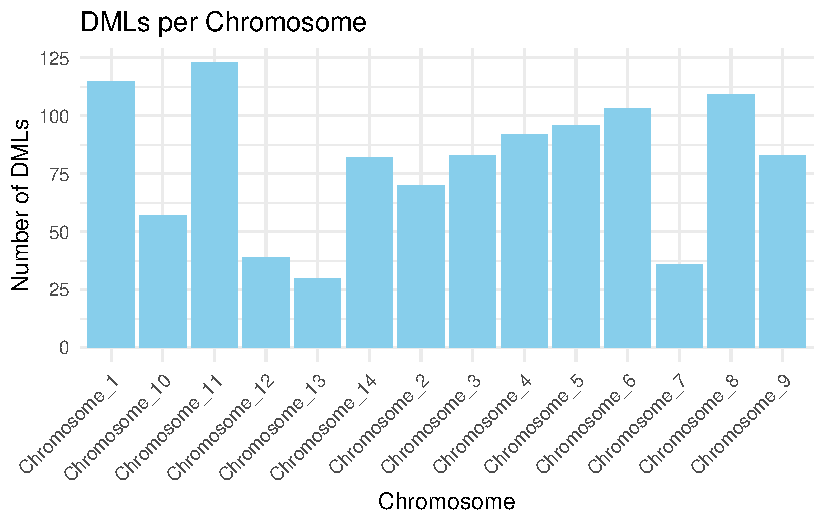
\includegraphics[keepaspectratio]{index_files/figure-pdf/unnamed-chunk-1-1.pdf}}

\textsubscript{Source:
\href{https://sr320.github.io/paper-chilean-mussel/index.qmd.html}{Article
Notebook}}

\subsection{Location}\label{location}

\begin{figure}[H]

{\centering \pandocbounded{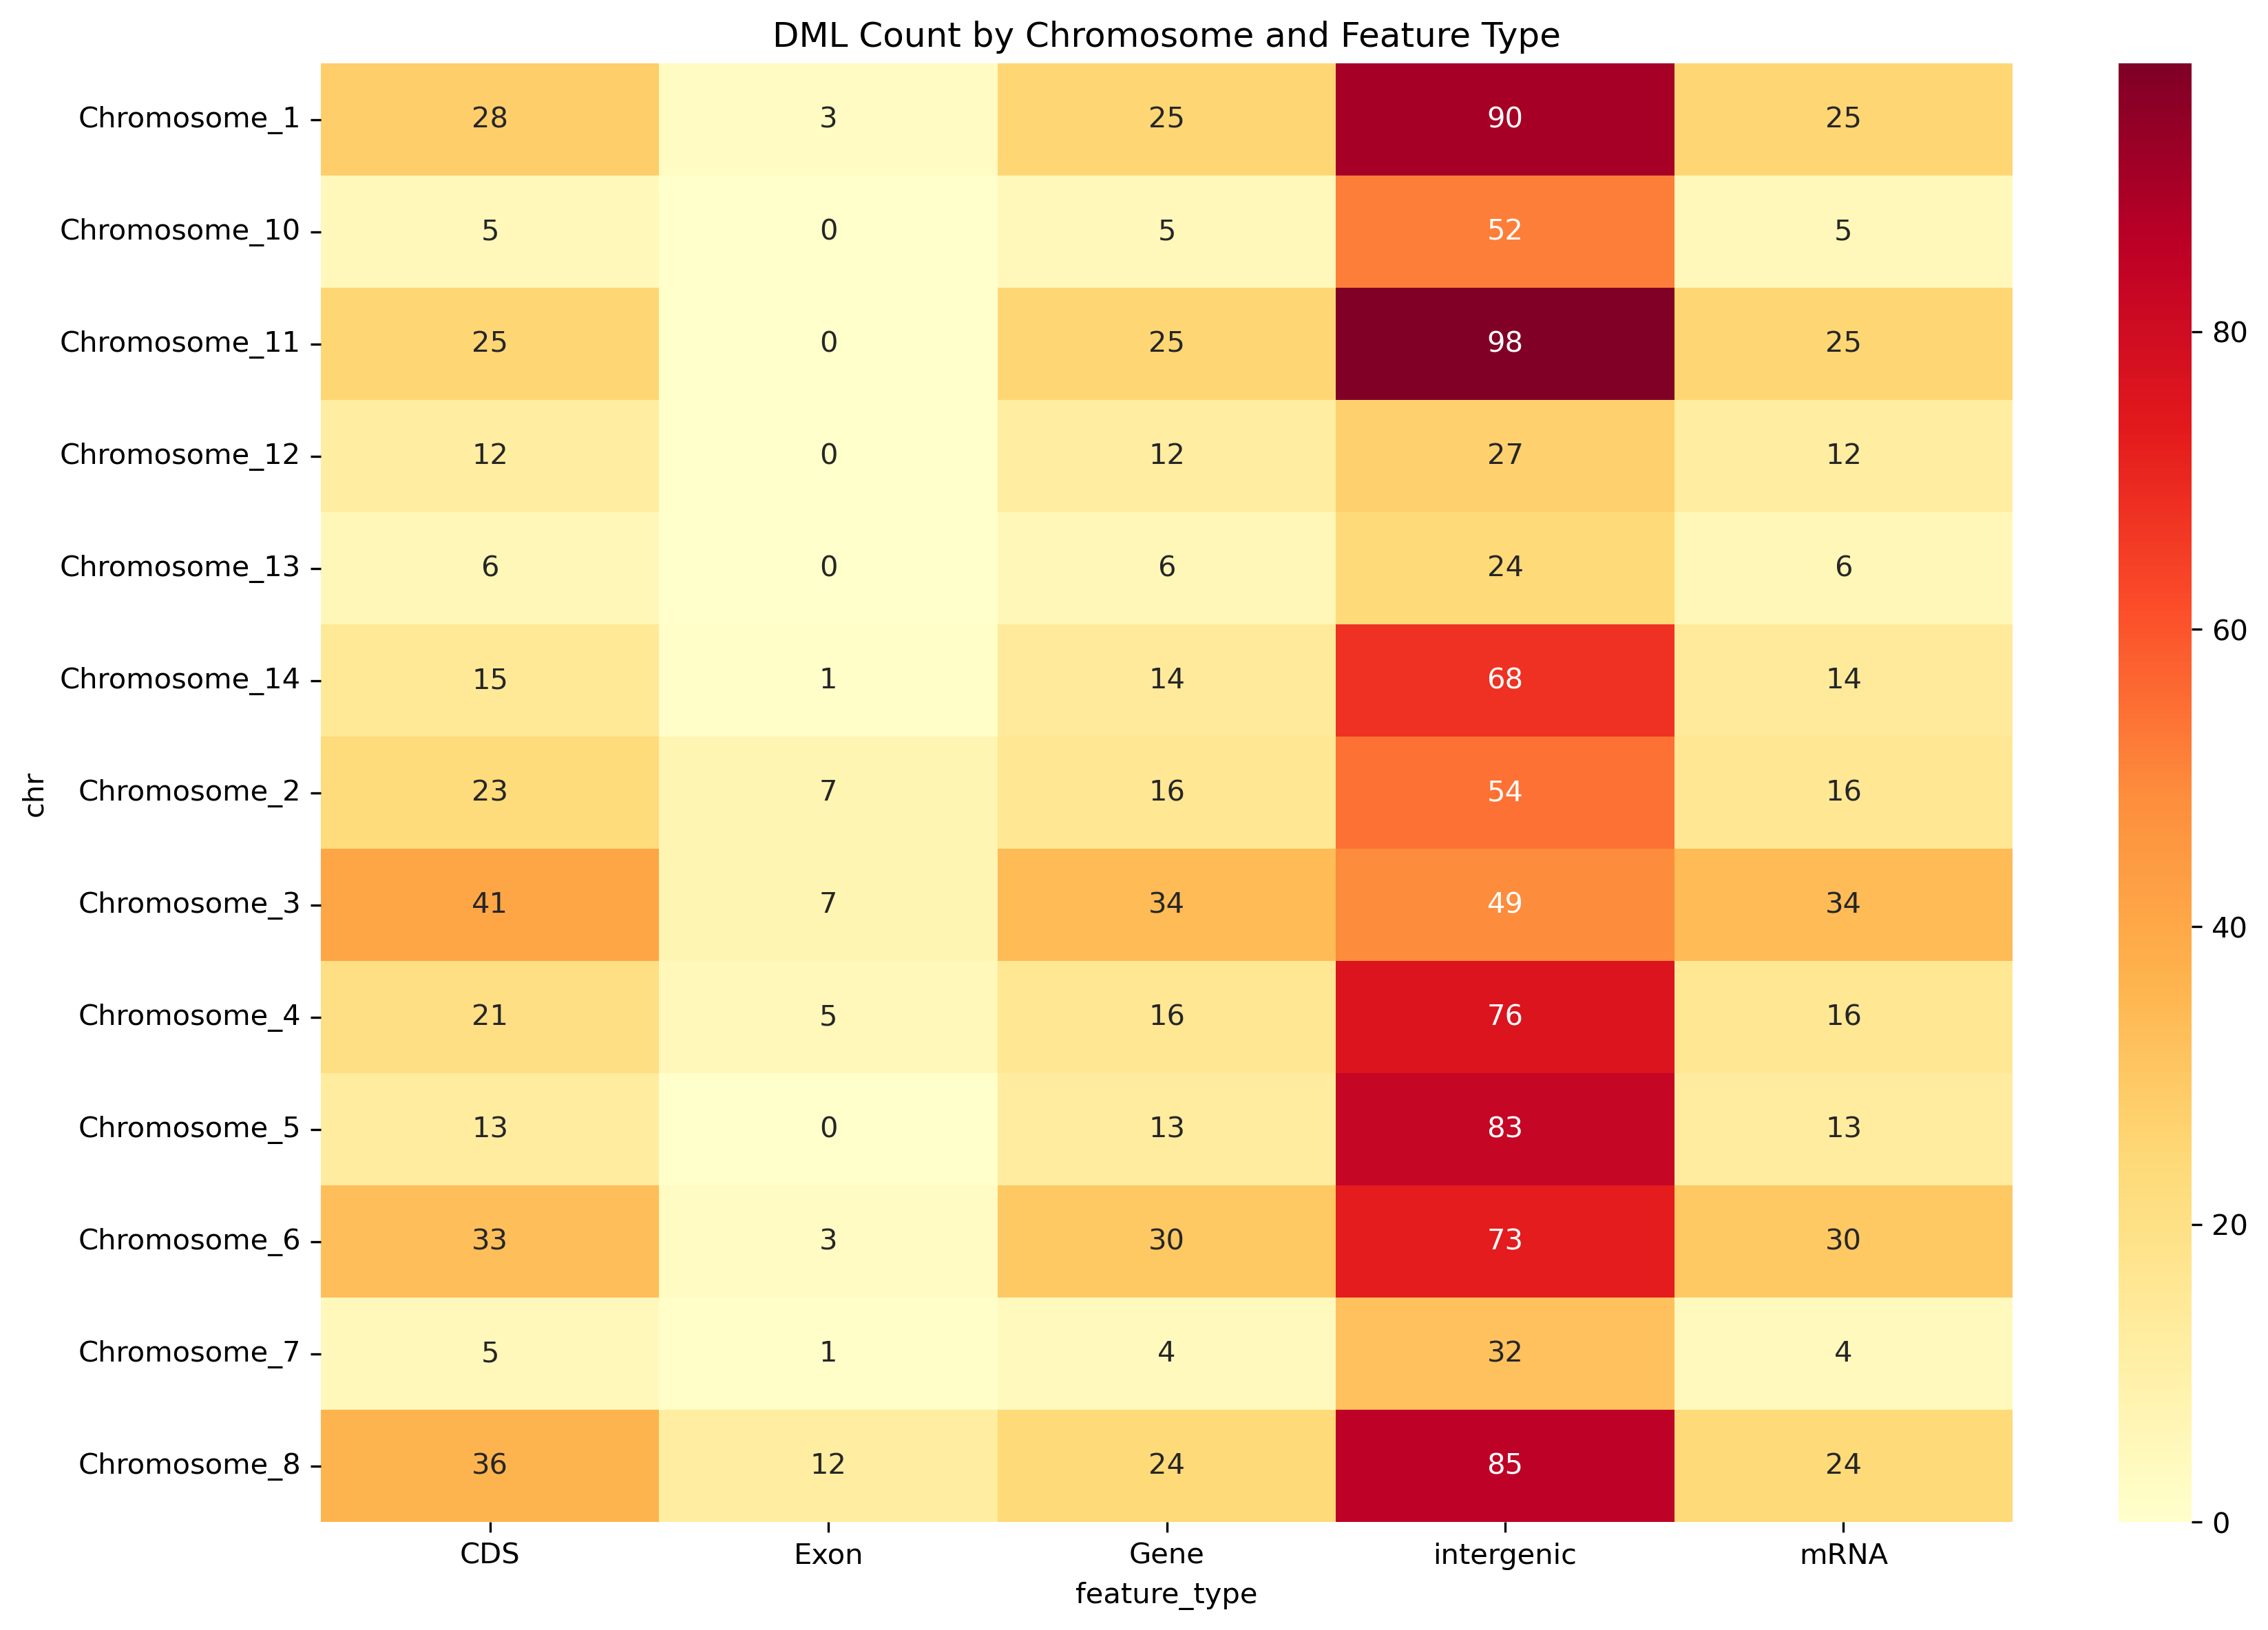
\includegraphics[keepaspectratio]{images/dml-heatmap.png}}

}

\caption{heatmap}

\end{figure}%

\subsection{Genes harboring DMLs and overall methylation
pattern}\label{genes-harboring-dmls-and-overall-methylation-pattern}

We identified 159 genes containing differentially methylated loci
(DMLs). For each gene, methylation differences were calculated by
aggregating the absolute methylation change at all DMLs mapped to that
gene, using the output from methylKit's logistic regression analysis.
Summary statistics (range: −77.04\% to +66.86\%; SD 40.48\%, median:
−8.96\%, mean: −0.68\%) were computed across these gene-level aggregated
values, indicating a shift toward hypomethylation among DML-associated
genes.

\subsection{Gene Ontology (GO): processes, functions, and
locations}\label{gene-ontology-go-processes-functions-and-locations}

Across Biological Process terms, DML genes were most frequently
annotated to metabolic process (71 genes; 44.7\% of all DML genes) and
to high-level developmental and cellular organization/biogenesis
categories (each 57 genes; 35.8\%). Additional frequent terms included
nitrogen compound metabolic process (63 genes; 39.6\%) and positive
regulation of biological process (57 genes; 35.8\%). For Molecular
Function, broad binding categories predominated (binding: 81 genes,
50.9\%; protein binding: 58 genes, 36.5\%), consistent with an
overrepresentation of regulatory and interaction-prone proteins.
Cellular Component assignments placed many targets in cell/intracellular
compartments (cell: 104 genes, 65.4\%; intracellular: 99 genes, 62.3\%),
with frequent localization to the cytoplasm (80 genes, 50.3\%) and
nucleus (53 genes, 33.3\%)

These patterns indicate that DMLs are concentrated in genes mediating
metabolism, developmental programs, and cellular organization, with many
targets residing in cytoplasmic and nuclear contexts where gene
regulation and signal processing occur.

\subsection{KEGG pathways}\label{kegg-pathways}

DML-associated genes mapped to 122 unique KEGG pathways, with most
pathways represented by a single gene, reflecting broad functional
dispersion rather than concentration in a small number of routes.
Prominent pathway classes included amino acid, carbohydrate, lipid, and
nucleotide metabolism, as well as signal transduction and cellular
process categories. The prevalence of core metabolic routes aligns with
the GO-based enrichment of metabolic processes and suggests potential
epigenetic modulation of energy balance and biosynthesis.

\subsection{Pfam domains}\label{pfam-domains}

We detected 118 unique Pfam domains among DML-associated genes,
generally with low redundancy (most domains present in one or two
genes), underscoring protein family diversity. Recurrently observed
domains included the RNA recognition motif (PF00076)---implicating
post-transcriptional regulation---alongside regulatory/interaction
modules such as BTB/POZ (PF07707) and ankyrin repeats (PF00023). We also
observed immunoglobulin domains (PF00047) and cytochrome P450 families
(PF00061/ PF00067), the latter consistent with roles in xenobiotic and
lipid metabolism. Several domains of unknown function (DUFs) were
present, indicating potentially novel or poorly characterized targets of
methylation.

\subsection{Directionality of methylation
changes}\label{directionality-of-methylation-changes}

Given the negative median methylation difference, hypomethylation was
more common among DML genes. Functionally, hypomethylated targets were
enriched for regulatory proteins, signaling molecules, and transporters,
whereas hypermethylated targets included transcription factors,
metabolic enzymes, and structural proteins. Collectively, these patterns
are consistent with widespread epigenetic remodeling across regulatory
and metabolic layers, rather than changes confined to a single pathway
or compartment.

\subsection{Summary}\label{summary}

Together, these results show that genes harboring DMLs in Mytilus
chilensis are functionally diverse. However, they converge on
metabolism, development, and cellular organization, with many targets
positioned in cytoplasmic and nuclear environments. The distribution of
DMLs is skewed toward hypomethylation. DML-associated genes are
dispersed across many KEGG pathways and contain regulatory or
interaction-rich Pfam domains. These findings suggest a system-wide
epigenetic response with potential consequences for metabolic control
and developmental programming.

\phantomsection\label{refs}
\begin{CSLReferences}{1}{0}
\bibitem[\citeproctext]{ref-castillo2017ocean}
Castillo, N., Saavedra, L. M., Vargas, C. A., Gallardo-Escárate, C., \&
Détrée, C. (2017). Ocean acidification and pathogen exposure modulate
the immune response of the edible mussel *mytilus chilensis*. \emph{Fish
\& Shellfish Immunology}, \emph{70}, 149--155.
\url{https://doi.org/10.1016/j.fsi.2017.08.047}

\bibitem[\citeproctext]{ref-montufar2024hypoxia}
Montúfar-Romero, M., Valenzuela-Muñoz, V., Valenzuela-Miranda, D., \&
Gallardo-Escárate, C. (2024). Hypoxia in the blue mussel *mytilus
chilensis* induces a transcriptome shift associated with endoplasmic
reticulum stress, metabolism, and immune response. \emph{Genes},
\emph{15}(6), 658. \url{https://doi.org/10.3390/genes15060658}

\bibitem[\citeproctext]{ref-montufar2025microbiota}
Montúfar-Romero, M., Valenzuela-Miranda, D., Valenzuela-Muñoz, V.,
Morales-Rivera, M. F., \& Gallardo-Escárate, C. (2025). Microbiota
dysbiosis in *mytilus chilensis* is induced by hypoxia, leading to
molecular and functional consequences. \emph{Microorganisms},
\emph{13}(4), 825. \url{https://doi.org/10.3390/microorganisms13040825}

\bibitem[\citeproctext]{ref-yevenes2021adaptive}
Yévenes, M., Núñez-Acuña, G., Gallardo-Escárate, C., \& Gajardo, G.
(2021). Adaptive differences in gene expression in farm-impacted
seedbeds of the native blue mussel *mytilus chilensis*. \emph{Frontiers
in Genetics}, \emph{12}, 666539.
\url{https://doi.org/10.3389/fgene.2021.666539}

\bibitem[\citeproctext]{ref-yevenes2022adaptive}
Yévenes, M., Núñez-Acuña, G., Gallardo-Escárate, C., \& Gajardo, G.
(2022). Adaptive mitochondrial genome functioning in ecologically
different farm-impacted natural seedbeds of the endemic blue mussel
*mytilus chilensis*. \emph{Comparative Biochemistry and Physiology Part
D: Genomics and Proteomics}, \emph{42}, 100955.
\url{https://doi.org/10.1016/j.cbd.2021.100955}

\bibitem[\citeproctext]{ref-yevenes2023epigenetic}
Yévenes, M., Gallardo-Escárate, C., \& Gajardo, G. (2023). Epigenetic
variation mediated by lncRNAs accounts for adaptive genomic
differentiation of the endemic blue mussel *mytilus chilensis*.
\emph{Heliyon}, \emph{10}(1), e23695.
\url{https://doi.org/10.1016/j.heliyon.2023.e23695}

\bibitem[\citeproctext]{ref-yevenes2025decoding}
Yévenes, M., Gajardo, G., \& Gallardo-Escárate, C. (2025). Decoding
local adaptation in the exploited native marine mussel *mytilus
chilensis*: Genomic evidence from a reciprocal transplant experiment.
\emph{International Journal of Molecular Sciences}, \emph{26}(3), 931.
\url{https://doi.org/10.3390/ijms26030931}

\end{CSLReferences}




\end{document}
